\documentclass[../../main.tex]{subfiles}
\begin{document}

\subsection*{3.2}
Una carica è distribuita all'interno di una sfera di raggio R con densità non uniforme $\rho (r) = c / r$ essendo c una costante.
\\Determinare le espressioni del campo elettrostatico E(x)e del potenziale V(r) per $0 \le r \le \infty$.
\\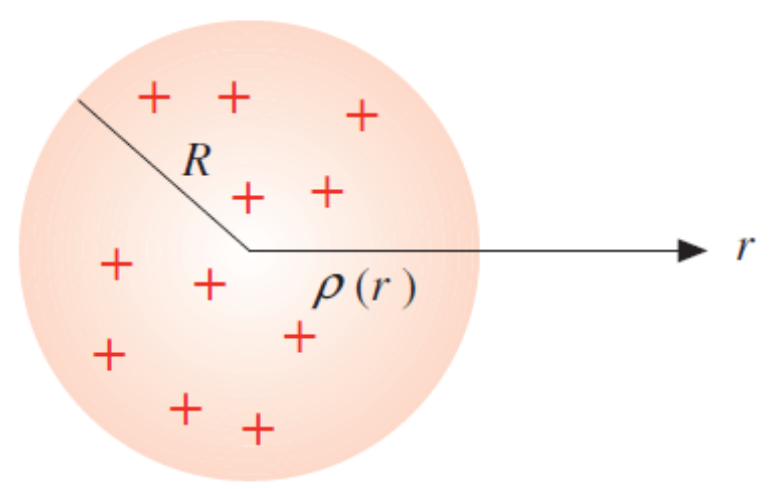
\includegraphics[scale=0.3]{e_3_2.png}
\subsubsection*{Formule utilizzate}
Gauss: $\Phi(\vec{E}) = \oint\vec{E}\vec{u_n}d\Sigma$
\subsubsection*{Soluzione punto a}
Gauss: $\Phi(\vec{E}) = \oint\vec{E}\vec{u_n}d\Sigma$ ma se $\vec{E} \parallel \vec{u_n} \rightarrow  \vec{E}\vec{u_n} = E$
\\$\Phi(\vec{E}) = \oint\vec{E}\vec{u_n}d\Sigma = \oint Ed\Sigma$ ma E è costante lungo $d\Sigma$
\\$\Phi(\vec{E}) = E\oint d\Sigma = E\Sigma$ con $\Sigma$ superfice sferica $\Sigma = 4\pi r^2$ 
\\$\Phi(\vec{E}) = E_r * 4\pi r^2$ con anche $\phi = \frac{q_{int}}{\epsilon_0}$
\\per $r \le R$ (interno sfera)
\\$4\pi r^2 E_{int} (x) = \frac{q_{int}(r)}{\epsilon_0}$
\\con $q_{int}(r) = \int_0^r \frac{c}{r}4\pi r^2dr = 2\pi cr^2$
\\$E_{int}(r) = \frac{C}{2\epsilon}$ costante
\\\\per $r > R$ (estero sfera)
\\$E_{est} = \frac{q}{4\pi \epsilon_0 r^2}$ con $q = 2\pi cR^2$
\\$E_{est} = \frac{cR^2}{2\epsilon_0 r^2}\ \ \ \ \ \ r(r \gg R) = \int_r^\infty E_{est}dr = \frac{cR^2}{2\epsilon_0 r}$
\\in particolare $V(R) = \frac{cR^2}{2\epsilon_0}$
\subsubsection*{Soluzione punto b}
per $ r\ll R$
\\$V(r) - V(R) = \int^R_rE_{int}dr = \frac{C}{2\epsilon_0}(R-r)$
\\$V(r) = \frac{c}{2\epsilon_0}(2R-r)$
\\al centro $V(0) = \frac{cR}{\epsilon_0}$ 
\newpage

\end{document}